%\usepackage{tikz}

% Tikz lines
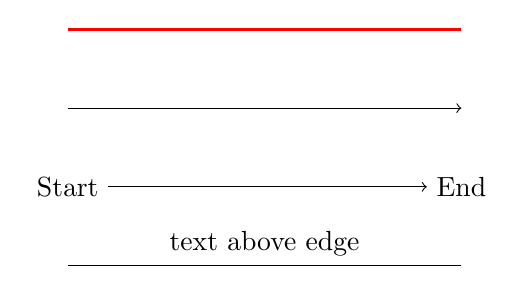
\begin{tikzpicture}
	\draw[red, very thick](0,0) -- (5,0);

	\draw[->] (0,-1) -- (5,-1);

	\node (1) at (0,-2) {Start};
	\node (2) at (5,-2) {End};
	\draw[->] (1) -- (2);

	\draw (0,-3) -- node[above] {text above edge} (5,-3);
\end{tikzpicture}

% Tikz shapes
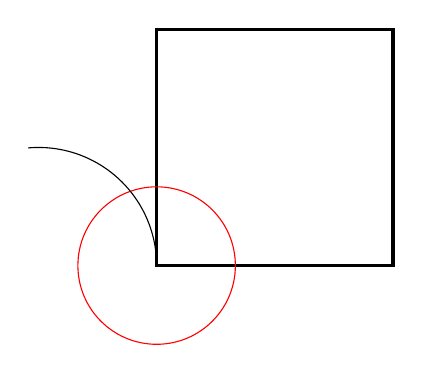
\begin{tikzpicture}
	\draw[very thick](0,0) rectangle (3,3);
	\draw[red](0,0) circle ();
	\draw(0,0) arc (0:95:1.5);
\end{tikzpicture}

% Tikz trees
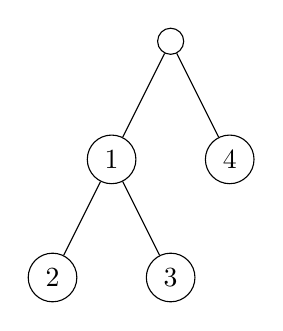
\begin{tikzpicture}[every node/.style={circle, draw=black}]
	\node{}
	child{node{1}
	child{node{2}}
	child{node{3}}}
	child{node{4}};
\end{tikzpicture}
